\documentclass[
10pt, % Set the default font size, options include: 8pt, 9pt, 10pt, 11pt, 12pt, 14pt, 17pt, 20pt
%t, % Uncomment to vertically align all slide content to the top of the slide, rather than the default centered
aspectratio=169, % Uncomment to set the aspect ratio to a 16:9 ratio which matches the aspect ratio of 1080p and 4K screens and projectors
]{beamer}

\usepackage[all]{xy}

\usepackage[spanish]{babel}
\usepackage[utf8]{inputenc}

\graphicspath{{Images/}{./}} % Specifies where to look for included images (trailing slash required)

\usepackage{booktabs} % Allows the use of \toprule, \midrule and \bottomrule for better rules in tables

%\usepackage{tikz}
%\usetikzlibrary{positioning}
%\usetikzlibrary{shapes,arrows,arrows,positioning,fit}

\usepackage{tikz}
\usepackage{adjustbox}
\usetikzlibrary{arrows, shapes}

\usepackage{forest}

\usepackage{multirow}

\usepackage{graphicx}
\usepackage{hyperref}

\usepackage{xcolor,listings}
\usepackage{textcomp}
%\usepackage{color}

\usepackage{enumitem}

\usepackage{xcolor}

\usepackage{verbatim}
\usepackage{changepage}

\usepackage{algorithm}
\usepackage{algpseudocode}
\usepackage{gensymb}

\usepackage{venndiagram}

\usepackage{graphicx}

\usepackage{array}

\usepackage{colortbl}
\usetikzlibrary{positioning}

\usepackage{pgfplots}

% \usepackage{media9}

% \usepackage{algorithm}
% \usepackage{algorithmic}

\providecommand{\abs}[1]{\lvert#1\rvert}

%----------------------------------------------------------------------------------------
%	SELECT LAYOUT THEME
%----------------------------------------------------------------------------------------
\usetheme{Madrid} 

%----------------------------------------------------------------------------------------
%	SELECT COLOR THEME
%----------------------------------------------------------------------------------------
%\usecolortheme{beaver}
%\usecolortheme{seahorse}
\usecolortheme{spruce} % verde suave
%\usecolortheme{whale}
%\usecolortheme{wolverine}

%----------------------------------------------------------------------------------------
%	SELECT FONT THEME & FONTS
%----------------------------------------------------------------------------------------
\usefonttheme{default} % Typeset using the default sans serif font
%\usefonttheme{serif} % Typeset using the default serif font (make sure a sans font isn't being set as the default font if you use this option!)
%\usefonttheme{structurebold} % Typeset important structure text (titles, headlines, footlines, sidebar, etc) in bold
%\usefonttheme{structureitalicserif} % Typeset important structure text (titles, headlines, footlines, sidebar, etc) in italic serif
%\usefonttheme{structuresmallcapsserif} % Typeset important structure text (titles, headlines, footlines, sidebar, etc) in small caps serif

%------------------------------------------------

%\usepackage{mathptmx} % Use the Times font for serif text
%\usepackage{palatino} % Use the Palatino font for serif text

\usepackage{helvet} % Use the Helvetica font for sans serif text
%\usepackage[default]{opensans} % Use the Open Sans font for sans serif text
%\usepackage[default]{FiraSans} % Use the Fira Sans font for sans serif text
\usepackage[default]{lato} % Use the Lato font for sans serif text

%----------------------------------------------------------------------------------------
%	SELECT INNER THEME
%----------------------------------------------------------------------------------------
\useinnertheme{circles}


\setbeamertemplate{footline} % Uncomment this line to remove the footer line in all slides
%\setbeamertemplate{footline}[page number] % Uncomment this line to replace the footer line in all slides with a simple slide count

\setbeamertemplate{navigation symbols}{} % Uncomment this line to remove the navigation symbols from the bottom of all slides

%----------------------------------------------------------------------------------------
%	PRESENTATION INFORMATION
%----------------------------------------------------------------------------------------

\title[Short Title]{Recuperación de información en conjuntos masivos} 

\subtitle{Sistemas de Recuperación de Información}

\author{Lic. Carlos León González \\ Dra.C. Lucina García Hernández}

\institute[UC]{Facultad de Matem\'atica y Computaci\'on \\ Universidad de La Habana \\ \smallskip }

\date{8 de julio de  2024} % Presentation date or conference/meeting name, the optional parameter can contain a shortened version to appear on the bottom of every slide, while the required parameter value is output to the title slide

%----------------------------------------------------------------------------------------

\begin{document}
	
	\lstset{
		literate=%
		{á}{{\'a}}1
		{í}{{\'i}}1
		{é}{{\'e}}1
		{ý}{{\'y}}1
		{ú}{{\'u}}1
		{ó}{{\'o}}1
		{ě}{{\v{e}}}1
		{š}{{\v{s}}}1
		{č}{{\v{c}}}1
		{ř}{{\v{r}}}1
		{ž}{{\v{z}}}1
		{ď}{{\v{d}}}1
		{ť}{{\v{t}}}1
		{ň}{{\v{n}}}1                
		{ů}{{\r{u}}}1
		{Á}{{\'A}}1
		{Í}{{\'I}}1
		{É}{{\'E}}1
		{Ý}{{\'Y}}1
		{Ú}{{\'U}}1
		{Ó}{{\'O}}1
		{Ě}{{\v{E}}}1
		{Š}{{\v{S}}}1
		{Č}{{\v{C}}}1
		{Ř}{{\v{R}}}1
		{Ž}{{\v{Z}}}1
		{Ď}{{\v{D}}}1
		{Ť}{{\v{T}}}1
		{Ň}{{\v{N}}}1                
		{Ů}{{\r{U}}}1    
	}
	
	
	\begin{frame}
		\titlepage
	\end{frame}
	
	%------------------------------------------------
	% Objetivos
	\begin{frame}
		
		\frametitle{Objetivos}
		
		\begin{itemize}
			
			\item Comprender el uso de Hadoop y MapReduce en el contexto de la recuperación de información para indexar, procesar y analizar grandes conjuntos de datos. \\[2mm]
			
			\item Explorar cómo la computación evolutiva puede ofrecer un enfoque innovador para resolver problemas complejos en el ámbito de la recuperación de información. 
			
		\end{itemize}
		
	\end{frame}
	
	%------------------------------------------------
	% Presencia de Big Data
	\begin{frame}
		
		\frametitle{Presencia de Big Data}
		
		\begin{alertblock}{}
			Conjuntos extremadamente grandes, complejos y diversos de datos que superan la capacidad de las herramientas tradicionales de procesamiento de datos para capturar, almacenar, gestionar y analizar de manera efectiva.
		\end{alertblock}
		
		% Las bases de datos relacionales y los software estadísticos tradicionales son ineficientes.
		
		% Con la explosión de las nuevas tecnologías como la computación en la nube, las redes móviles y la web semántica, hay un aumento de información a niveles incomprensibles.
		
		\centering
		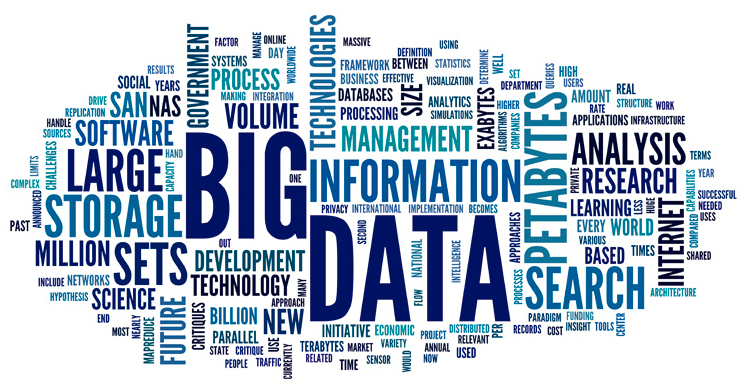
\includegraphics[scale=0.4]{big-data.png}
		
		{\scriptsize Tomado de 	\url{https://tdwi.org/articles/2020/03/03/adv-all-how-accounting-teams-can-leverage-big-data.aspx}}
		
		
	\end{frame}
	
	%------------------------------------------------
	%  Propiedades de Big Data
	\begin{frame}
		
		\frametitle{Propiedades de Big Data}
		
		
		\centering
		\vspace{6\baselineskip}
		{\scriptsize Tomado de 	\url{https://ed.team/comunidad/las-5-vand-39-s-del-big-data}}
		
	\end{frame}
	
	%------------------------------------------------
	% Propiedades de Big Data
	\begin{frame}
		
		\centering
		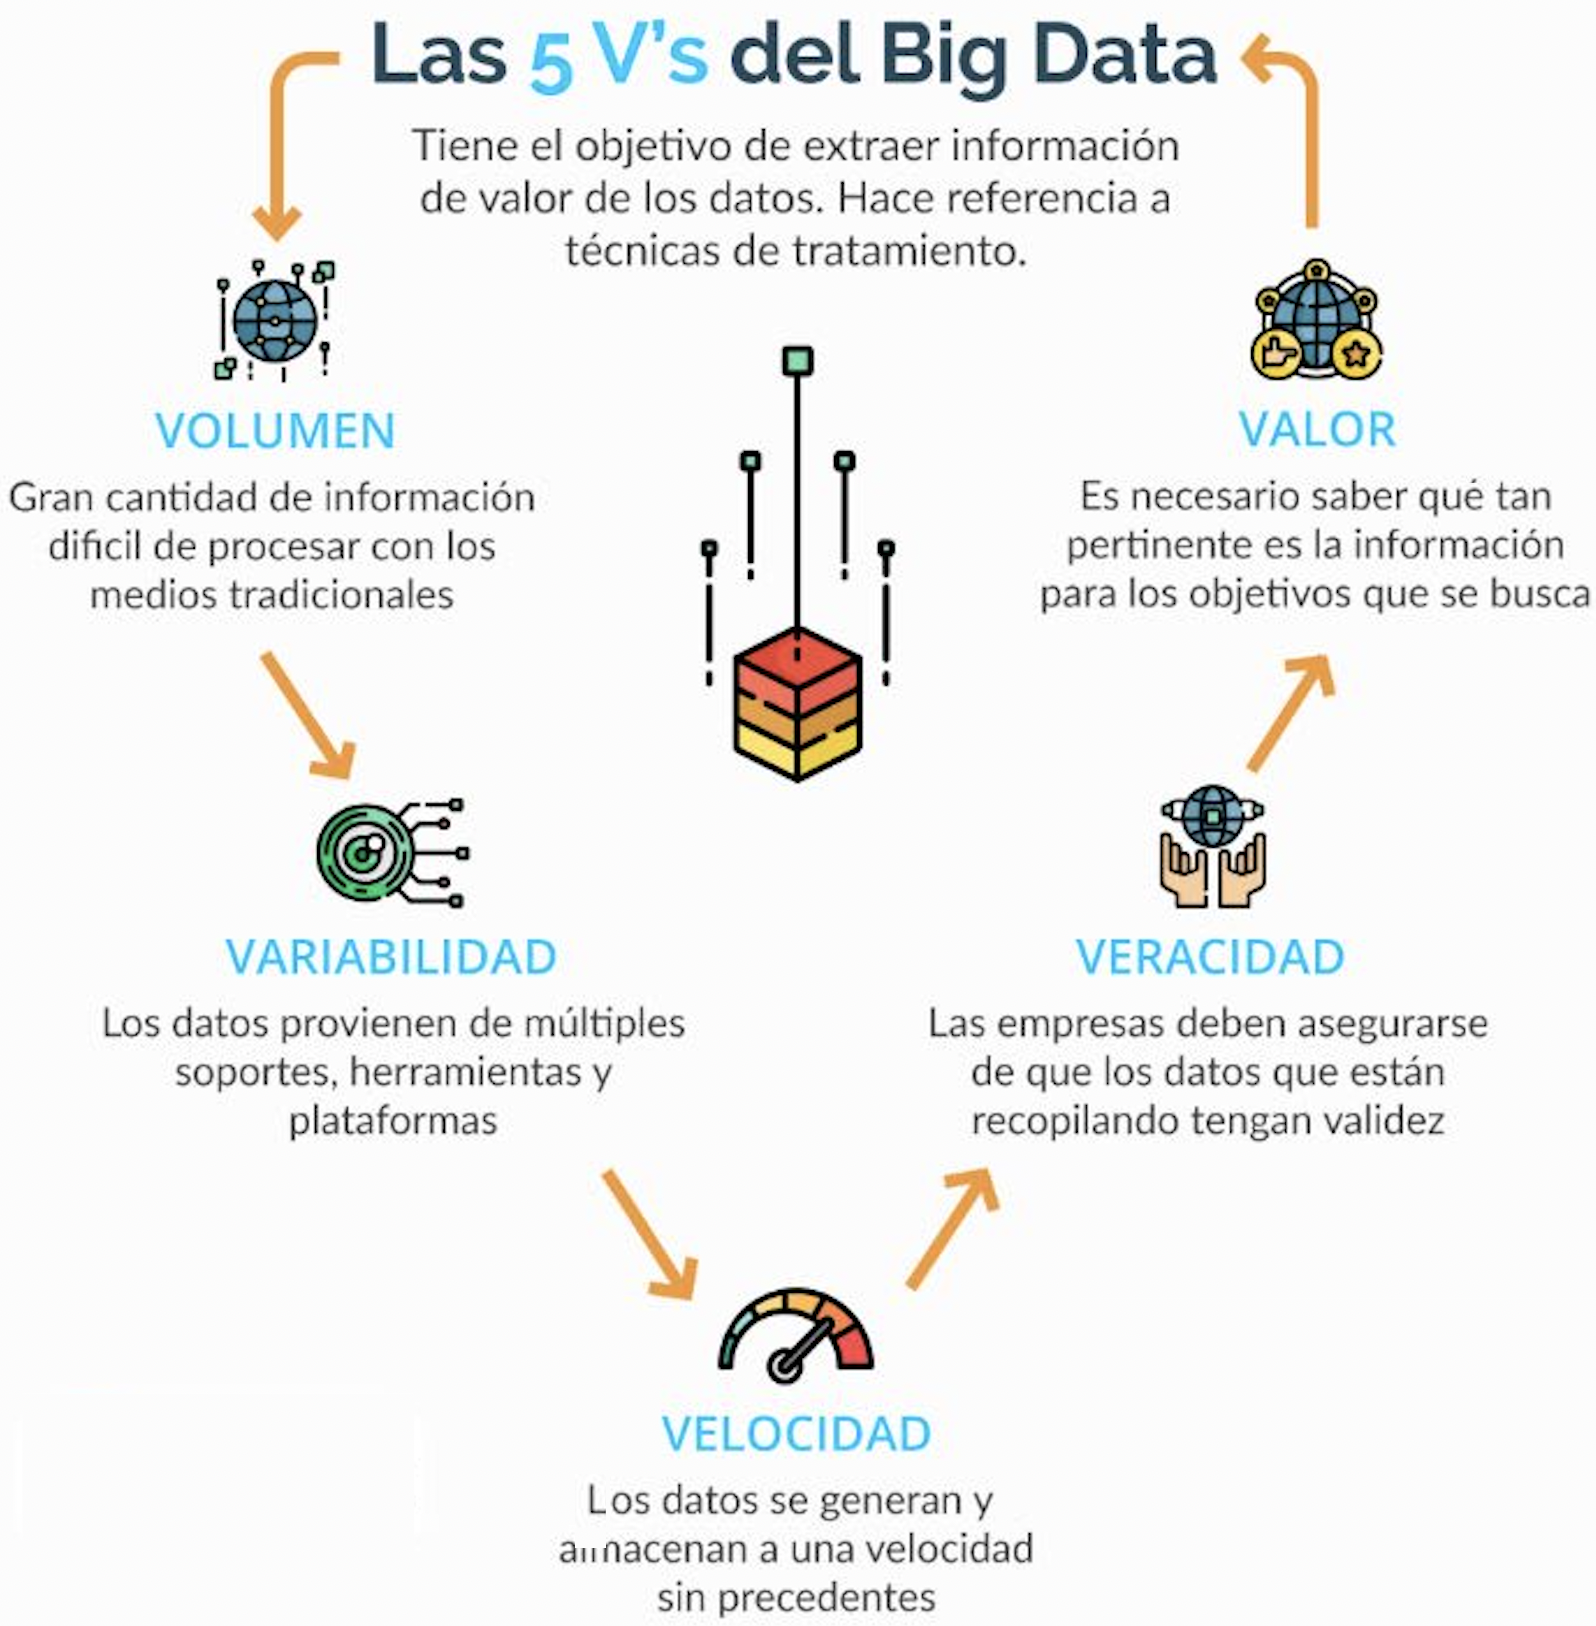
\includegraphics[height=\paperheight]{5-v-big-data.png}
		
		% Volumen 
		% 	Los datos provienen de diferentes fuentes y se encuentran en distintos formatos, creciendo exponencialmente cada día. La mayoría de los datos capturados provienen de web sociales.
		
		% Variabilidad 
		% 	Los datos se encuentran en distintos formatos y de naturaleza relacional, semiestracturada que incorporan datos XML y no estructurados que incorporan PDF, texto y otros medios. Cada dato tiene diferentes dimensiones por lo que extraer información relevante par su posterior procesamiento es una complicada tarea.
		
		% Velocidad 
		% 	La velocodad de creación de los datos es increiblemente alta, los cuales se acumulan en tiempo real a un ritmo rápido. Con la expansión de las redes sociales, un mensaje de varios minutos se considera obsoleto. Realizar análisis en tiempo real de un volumen tan alto de datos en movimiento y a través de todos los límites ayuda a revolucionar los sistemas de recuperación de información.
		
		% Veracidad 
		% 	Significa confiabilidad y comprensibilidad de los datos. Los datos deben producir el resultado de calidad deseado y ayudar a tomar la decisión correcta. Debe estar libre de discrepancias y ayudar a lograr el objetivo correcto.
		
		% Valor 
		% 	El objetivo final de cualquier tarea debe ser generar valor para que se pueda medir su relevancia. Este factor ayuda a extraer valor de los datos y proporcionar retorno de la inversión al brindar apoyo financiero futuro.
		
	\end{frame}
	
	%------------------------------------------------
	%  Motivación
	\begin{frame}
		
		\frametitle{Recordando el problema inicial}
		
		\centering
		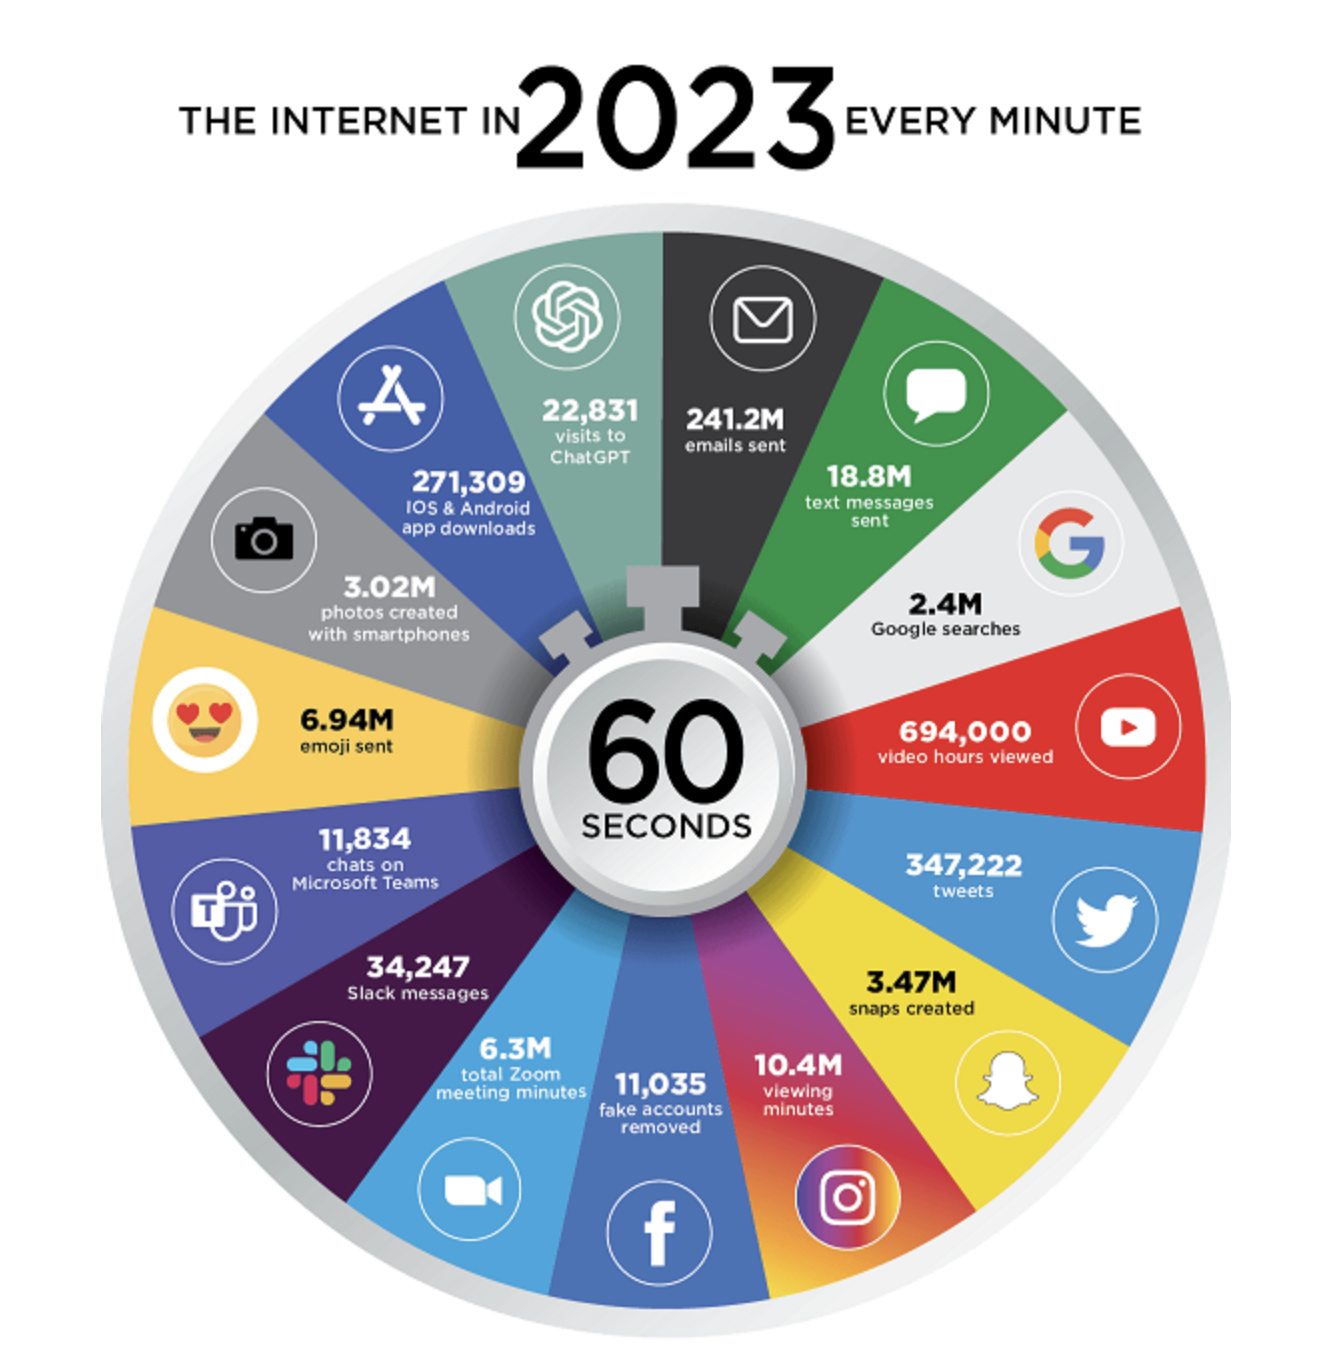
\includegraphics[scale=0.33]{infografia.png}
		
		% Características de lo datos:
		% 	- Datos heterogéneos.
		% 	- Distintas fuentes de datos.
		% 	- Datos volátiles.
		% 	- Damasiada información en un corto período de tiempo.
		
		% Se necesita:
		% 	- Minimizar el tiempo de las operaciones, sin perder la relevancia de los datos recuperados
		
	\end{frame}		
	
	%------------------------------------------------
	%  Motivación
	\begin{frame}
		
		\frametitle{Recordando el problema inicial}
		
		\begin{minipage}{.4\textwidth}
			
			Hay almacenado $24$ horas de toda la información. Entonces,  ¿cómo ...
			\begin{itemize}
				
				\item \textcolor{purple}{procesar o indexar los datos?} 
				
				\item \textcolor{purple}{buscar información?} 
				
				\item \textcolor{purple}{recuperar información?} 
				
			\end{itemize}
			
			\vspace{1\baselineskip}
			
			Cada proceso tiene que responder en el menor tiempo posible y como mínimo existe $10^6$ Gb de datos.
			
		\end{minipage}%
		\begin{minipage}{.7\textwidth}
			
			\centering
			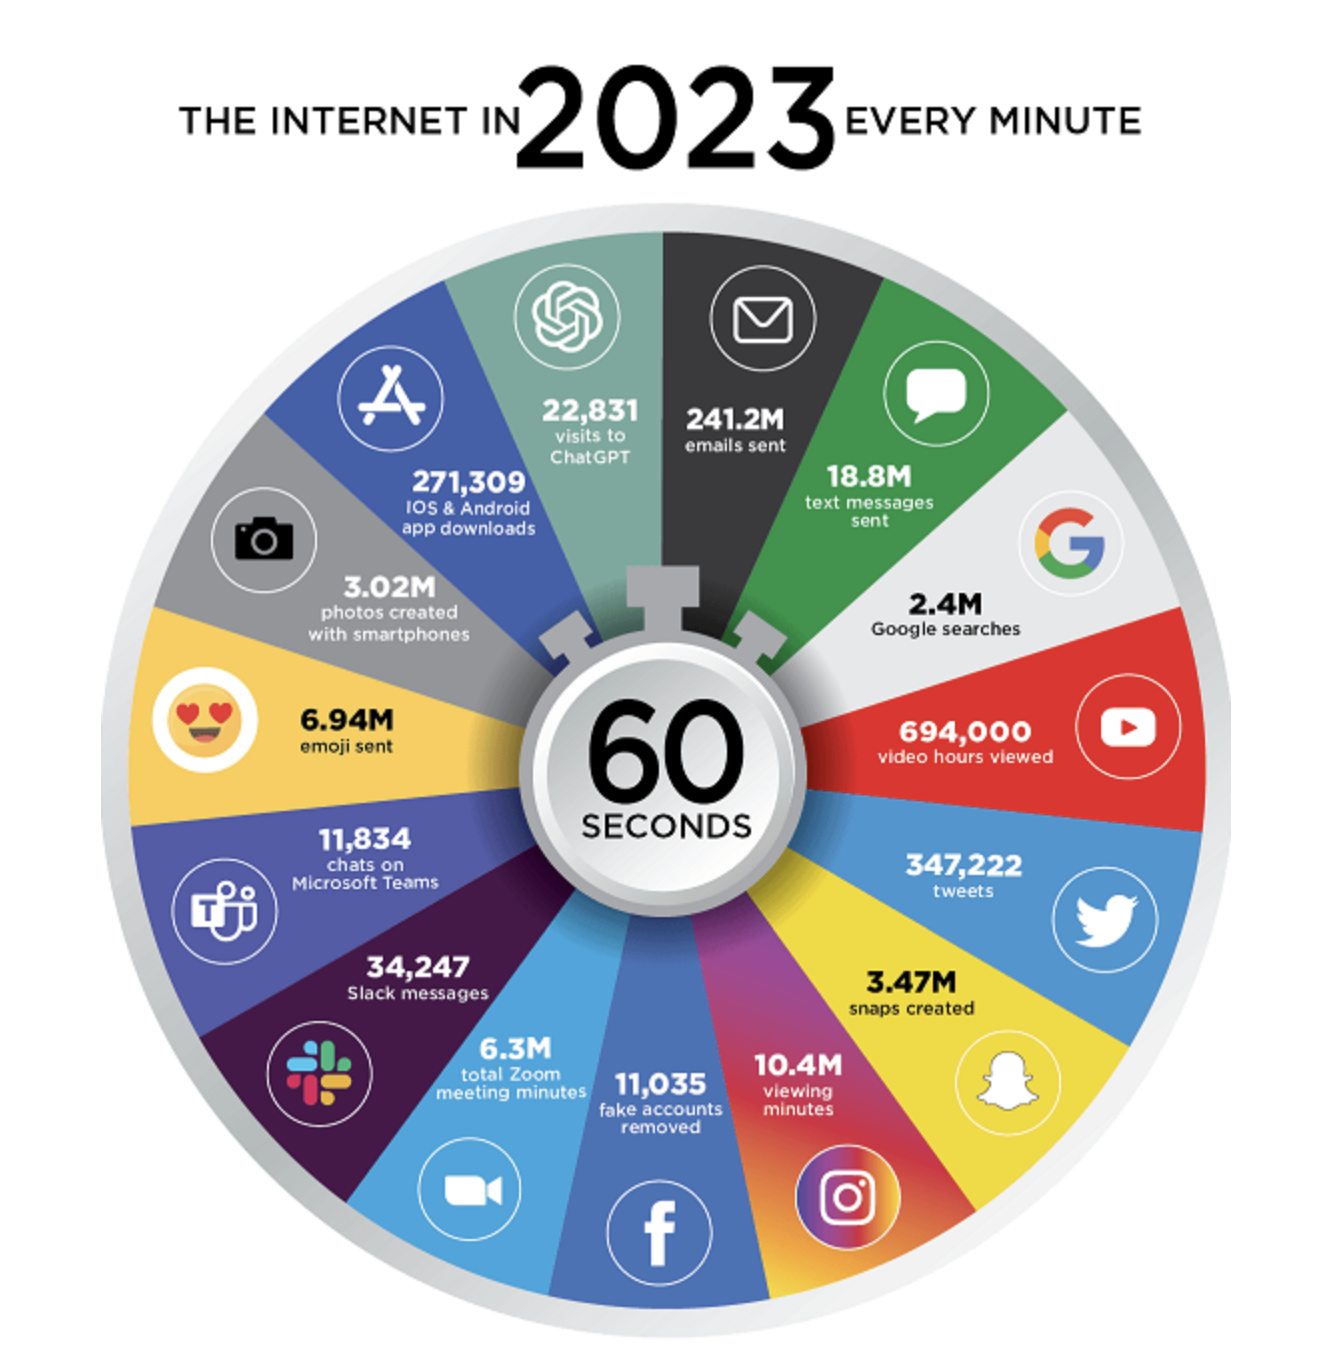
\includegraphics[scale=0.33]{infografia.png}
			
		\end{minipage}%
		
	\end{frame}
	
	%------------------------------------------------
	%  Posibles soluciones para disminuir el tiempo de cada proceso
	\begin{frame}
		
		\frametitle{Posibles soluciones para disminuir el tiempo de procesamiento}
		
		\begin{itemize}
			
			\item \textbf<3>{Paralelización} \\[2mm]
			% Dividir el proceso de análisis en tareas más pequeñas y ejecutarlas en paralelo en varios recursos de procesamiento, como múltiples núcleos de CPU, servidores distribuidos o clusters de computadoras. 
			
			\item \textbf<3>{Optimización de algoritmos} \\[2mm]
			% Revisar y optimizar los algoritmos utilizados en el proceso de análisis para garantizar que sean eficientes en términos de tiempo y recursos. Esto puede implicar la selección de algoritmos más rápidos, la optimización de algoritmos existentes o la implementación de técnicas de optimización específicas para el problema en cuestión.
			
			\item \textbf<3>{Uso de índices y estructuras de datos eficientes} \\[2mm]
			% Utilizar índices y estructuras de datos optimizados puede acelerar la búsqueda y recuperación de datos durante el análisis. Esto puede incluir el uso de índices de base de datos, estructuras de datos en memoria, como árboles o tablas hash, y técnicas de compresión de datos para reducir el tamaño de los conjuntos de datos.
			
			\item \textbf<3>{Uso de tecnologías de procesamiento de datos distribuidos} \\[2mm]
			% Adoptar tecnologías diseñadas específicamente para el procesamiento distribuido de datos, como Apache Hadoop, Apache Spark o sistemas de gestión de bases de datos distribuidas, puede ayudar a mejorar el tiempo de procesamiento al distribuir la carga de trabajo entre múltiples nodos de procesamiento.
			
			\item Utilización de hardware especializado \\[2mm]
			% Considerar el uso de hardware especializado, como unidades de procesamiento gráfico (GPU) o unidades de procesamiento de tensor (TPU), que están diseñadas específicamente para realizar cálculos intensivos en paralelo. Estos tipos de hardware pueden acelerar significativamente el tiempo de procesamiento para ciertas tareas, como el entrenamiento de modelos de aprendizaje automático o el procesamiento de imágenes.
			
			\item Escalamiento horizontal y vertical 
			% Escalar la infraestructura de procesamiento según sea necesario para manejar cargas de trabajo más grandes. Esto puede implicar agregar más recursos de procesamiento (escalamiento horizontal) o mejorar el rendimiento de los recursos existentes, como actualizar la CPU, la memoria o el almacenamiento (escalamiento vertical).
			
		\end{itemize}
		
		\only<2>{
			\vspace{3\baselineskip}
			\textcolor{purple}{¿Cuáles podemos garantizar desde la condición de ser programadores?}
		}
		
	\end{frame}
	
	%------------------------------------------------
	%  Apache
	\begin{frame}
		
		\frametitle{Apache Software Foundation}
		
		\centering
		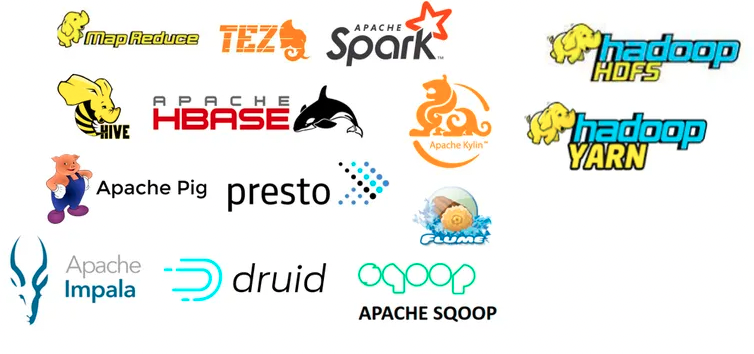
\includegraphics[scale=0.55]{apache.png}
		
		% Apache Software Foundation:
		% 	- organización proporciona un entorno colaborativo y neutral para el desarrollo de software de código abierto
		% 	- tiene licencia de software libre
		% 	- soporte de la comunidad
		% 	- énfases en la calidad y la seguridad
		% 	- infraestructura técnica y de recursos
		
		{\scriptsize Tomado de 	\url{https://juicefs.medium.com/from-hadoop-to-cloud-why-and-how-to-decouple-storage-and-compute-in-big-data-platforms-8e01e47e9ea0}}
		
	\end{frame}
	
	%------------------------------------------------
	%  Hadoop
	\begin{frame}
		
		\frametitle{Hadoop: Transformando el análisis de datos a escala}
		
		\begin{itemize}
			
			\item Herramienta básica. \\[3mm]
			 
			\item Opción viable para el procesamiento distribuido de grandes volúmenes de datos, especialmente para cargas de trabajo de procesamiento por lotes. \\[3mm]
			
			\item Componentes:
			\begin{itemize}
				\item YARN para la programación de recursos
				\item HDFS para almacenamiento de archivos distribuido
				\item MapReduce para el cálculo de los datos
				
			\end{itemize}
			
		\end{itemize}
		
	\end{frame}
	
	%------------------------------------------------
	%  Componentes de Hadoop
	\begin{frame}
		
		\frametitle{Componentes de Hadoop}
		
		\begin{itemize}
			\item YARN (Yet Another Resource Negotiator, Otro Negociador de Recursos) \\[3mm]
			
			Características:
			\begin{itemize}
				
				\item Gestión de recursos \\[1mm]
				% YARN gestiona los recursos de los clústeres, como la CPU y la memoria, y asigna estos recursos a las aplicaciones que se ejecutan en el clúster.
				
				\item Planificación de tareas \\[1mm]
				% YARN es responsable de la planificación de tareas y la asignación de recursos para las aplicaciones que se ejecutan en el clúster. Utiliza un modelo de planificación basado en contenedores para garantizar una utilización eficiente de los recursos.
				
				\item Soporte para múltiples marcos de procesamiento \\[1mm]
				% YARN permite la ejecución de múltiples frameworks de procesamiento, como MapReduce, Apache Spark, Apache Flink y otros, en el mismo clúster, lo que proporciona una mayor flexibilidad y capacidad de procesamiento.
				
				\item Escalabilidad \\[1mm]
				% YARN está diseñado para escalar de manera eficiente con el tamaño del clúster y el volumen de trabajo. Puede manejar clústeres de gran tamaño y grandes volúmenes de datos de manera efectiva.
				
			\end{itemize}
			
		\end{itemize}
		
	\end{frame}
	
	%------------------------------------------------
	%  
	\begin{frame}
		
		\frametitle{Componentes de Hadoop}
		
		\begin{itemize}
			\item Sistema de fichero distribuido (HDFS)\\[2mm]
			
			Características:
			\begin{itemize}
				
				\item Diseñado para ser altamente escalable 
				% HDFS está diseñado para ser altamente escalable y puede manejar grandes volúmenes de datos. Puede escalar horizontalmente agregando más nodos al clúster para aumentar su capacidad de almacenamiento.
				
				\item Tolerancia a fallos
				% HDFS proporciona una alta tolerancia a fallos al replicar los datos en múltiples nodos en el clúster. Por defecto, cada bloque de datos se replica en tres nodos diferentes para garantizar la disponibilidad de los datos en caso de fallo de un nodo.
				
				\item Modelo de acceso de datos \\[2mm]
				% HDFS ofrece un modelo de acceso de datos de tipo lectura-escritura. Los archivos se escriben una vez y luego se leen muchas veces. Esto lo hace adecuado para aplicaciones que requieren acceso a grandes conjuntos de datos, como procesamiento de datos en lotes, análisis de datos y almacenamiento de datos en bruto.
				
			\end{itemize}
			
			\centering
			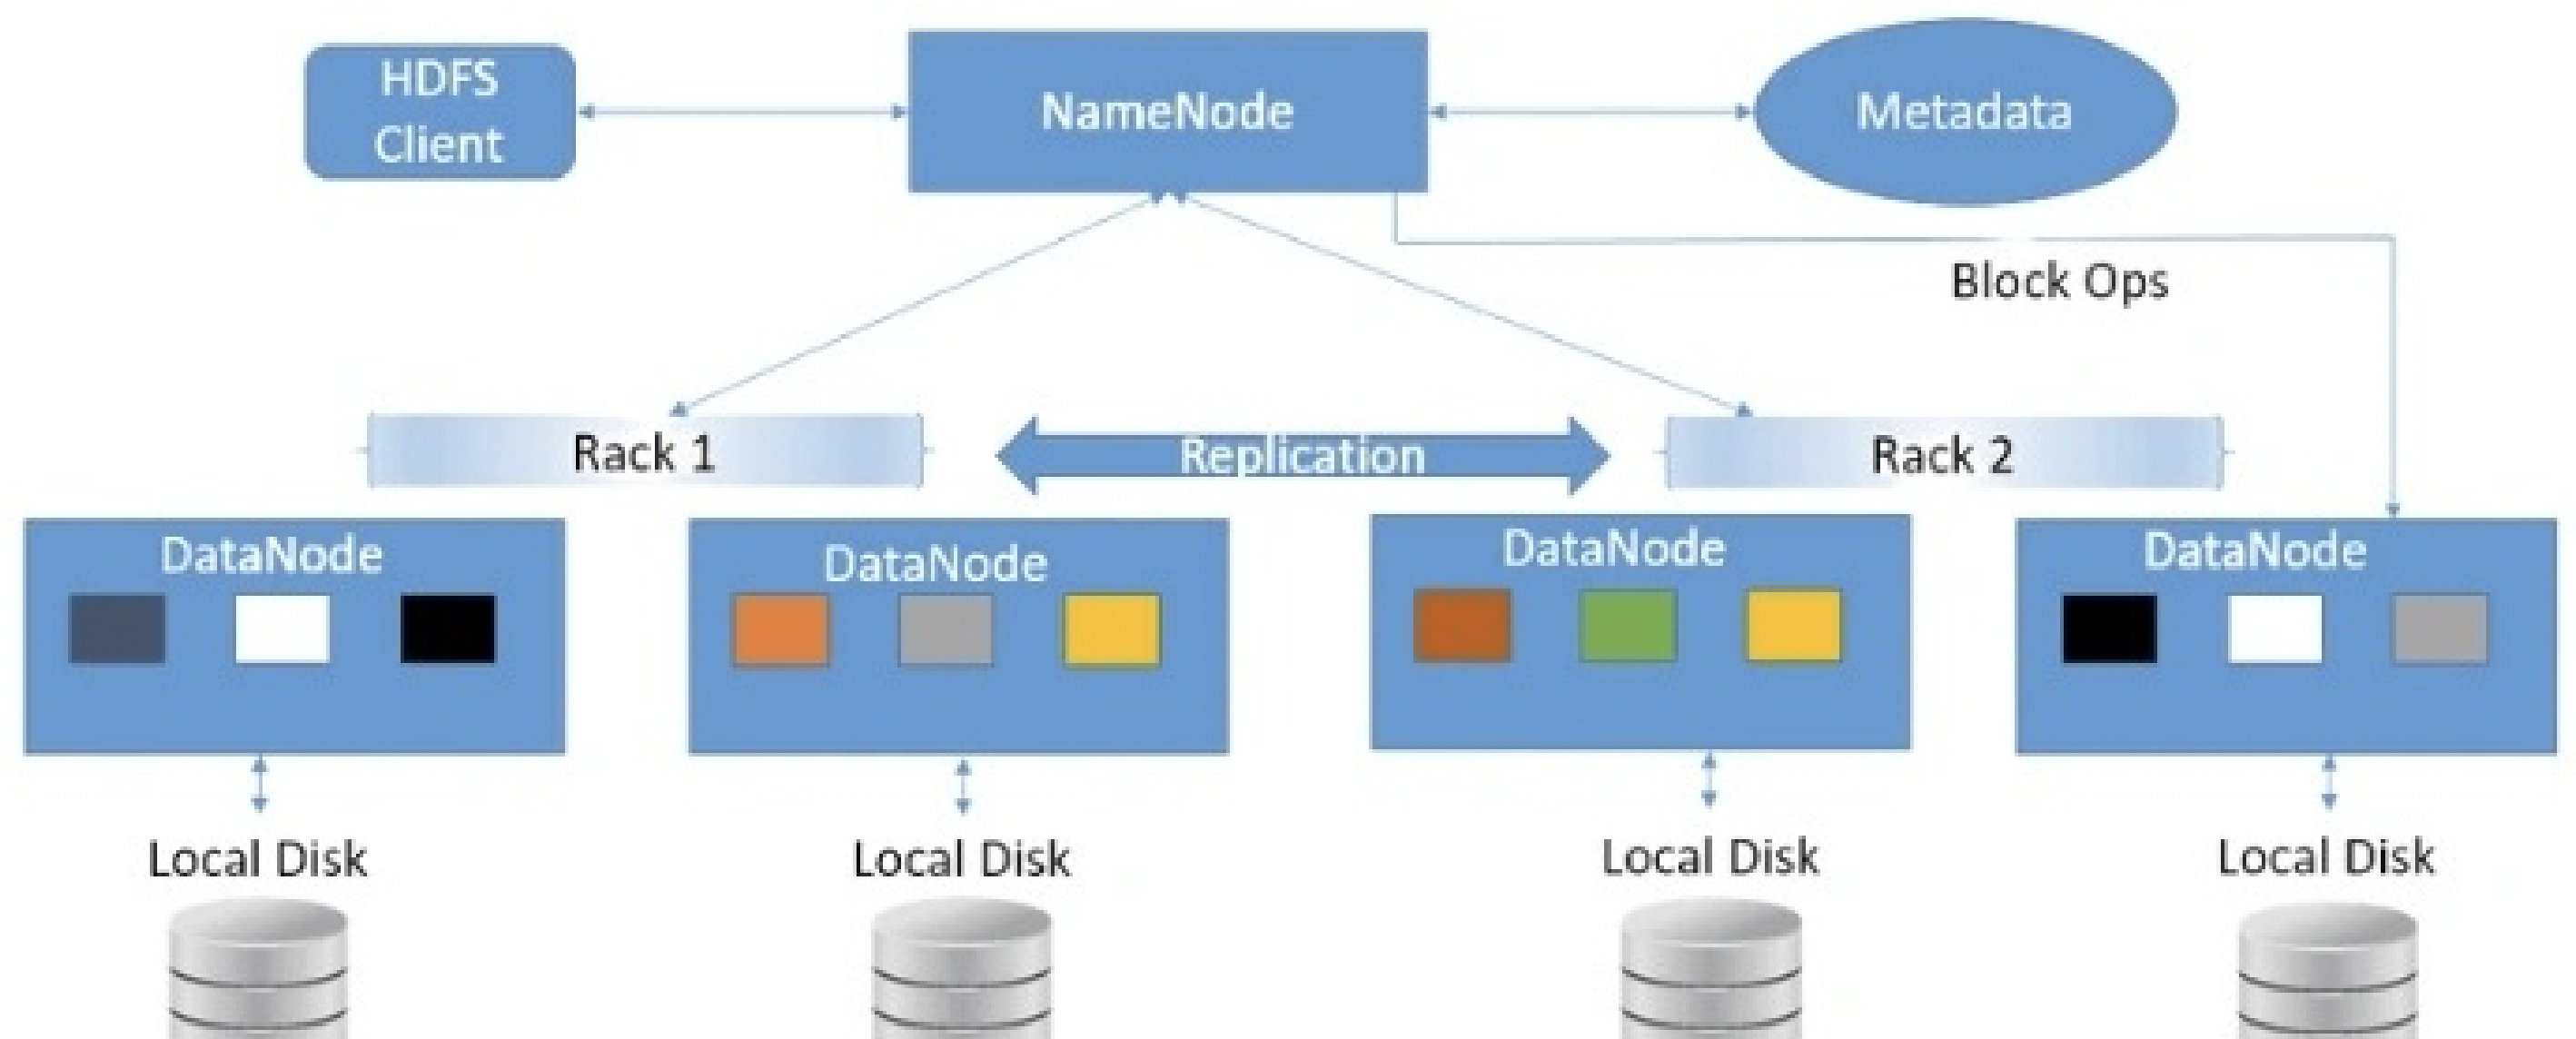
\includegraphics[scale=0.24]{hdfs.png}
			
			% ¿Cómo funciona?
			% 	1. Arquitectura de Nodo Maestro y Nodos de Datos
			% 		- sigue un modelo de arquitectura maestro-esclavo. 
			% 		- hay un nodo maestro llamado NameNode y varios nodos de datos llamados DataNodes. 
			% 		- NameNode es responsable de la gestión del sistema de archivos y mantiene un registro de la ubicación y los metadatos de todos los archivos en el clúster, mientras que los DataNodes almacenan los bloques de datos y gestionan su lectura y escritura.
			% 	2. Acceso de Datos y Operaciones de Archivos
			% 		- los clientes acceden a los archivos a través de una variedad de interfaces, como la interfaz de línea de comandos (CLI), APIs de programación y herramientas de gestión de archivos. 
			% 		- los clientes pueden leer, escribir, eliminar y manipular archivos y directorios en HDFS utilizando estas interfaces.
			
			{\scriptsize Tomado de 	\url{https://www.integrate.io/blog/guide-to-hdfs-for-big-data-processing/}}
			
		\end{itemize}
		
	\end{frame}
	
	%------------------------------------------------
	%  
	\begin{frame}
		
		\frametitle{Componentes de Hadoop}
		
		\begin{itemize}
			\item MapReduce \\[3mm]
			
			Características: 
			\begin{itemize}
				
				\item Basado en el modelo de programación funcional distribuida \\[2mm]
				
				\item Utilizado para procesar grandes volúmenes \\[2mm]
				% Por lo general se encuentra en clústeres que implementan algoritmos distribuidos y en paralelo para obtener los datos almacenados.
				
				\item Es altamente escalable \\[2mm]
				
				\item Abstracción de la programación distribuida \\[2mm]
				% Oculta la complejidad de la programación distribuida al proporcionar una abstracción de alto nivel para el procesamiento paralelo de datos.
				
				\item Compuesto por las funciones: 
				\begin{itemize}
					\item Map: realiza las tareas de filtrado y clasificación. \\[1mm]
					
					\item Reduce: realiza el resumen de los resultados.
				\end{itemize}
				
			\end{itemize}
			
		\end{itemize}		
		
	\end{frame}
	
	%------------------------------------------------
	%  MapReduce
	\begin{frame}
		
		\frametitle{Arquitectura de un programa con MapReduce}
		
		\centering
		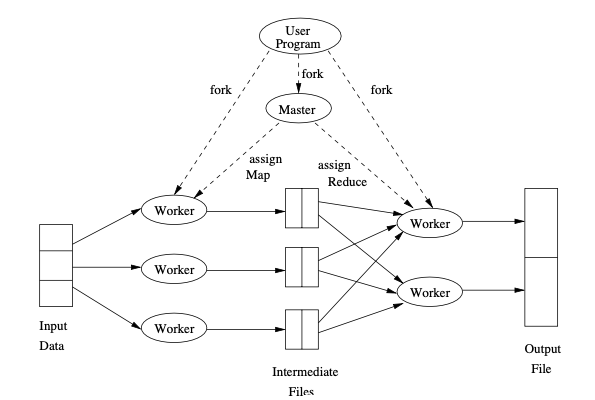
\includegraphics[scale=0.55]{arquitectura-map-reduce.png}
		
		% Pasos:
		% 	1. El sistema toma información del sistema de archivos y la divide en nodos de mapa separados.
		% 	2. La función o código del mapa se ejecuta y genera una salida para cada nodo del mapa.
		% 	3. Esta salida representa un conjunto de pares clave/valor intermedios que se mueven a nodos reducidos como entrada.
		% 	4. La función o código de reducción se ejecuta y genera una salida para cada nodo de reducción.
		% 	5. El sistema toma una salida de cada nodo para agregar una vista final.
		
		% Cada clúster puede tener implementado cualquier modelo de RI.
		
	\end{frame}
	
	%------------------------------------------------
	%  Break
	\begin{frame}
		
		\centering
		
\includegraphics[height=\paperheight]{break1.jpg}
		
	\end{frame}
	
	%------------------------------------------------
	%  Últimas interrogantes 
	\begin{frame}
		
		\frametitle{Últimas interrogantes}
		
		Hadoop, o el ecosistema de Apache en su totalidad, permite mejorar el procesamiento de los datos en Big Data, pero ... 
		
		\vspace{2\baselineskip}
				
		\textcolor{purple}{¿Basta con lo presentado para finalizar la búsqueda a mejorar el procesamiento y la recuperación de información en conjuntos de datos masivos?}
		
		\vspace{1\baselineskip}
		
		\textcolor{purple}{¿Qué no se ha analizado aun?}
		
		% Algoritmos para encontrar soluciones óptimas 
		
	\end{frame}
	
	%------------------------------------------------
	%  Computación evolutiva
	\begin{frame}
		
		\frametitle{Computación evolutiva}
		
		\begin{alertblock}{}
			Se refiere a sistemas de resolución de problemas que emplean modelos computacionales (algoritmos de optimización) basados en conceptos evolutivos para resolver problemas complejos y encontrar soluciones eficientes.
		\end{alertblock}
		
		% Los algoritmos evolutivos imitan el proceso de selección natural, donde se generan y evalúan soluciones candidatas, y las soluciones más aptas son seleccionadas y combinadas para producir nuevas soluciones en generaciones sucesivas. Este proceso de generación, evaluación y selección se repite iterativamente hasta encontrar una solución satisfactoria o hasta que se cumpla algún criterio de terminación.
		
		\vspace{1.5\baselineskip}
		
		Algoritmos utilizados para la RI en Big Data:
		\begin{itemize}
			\item Algoritmo genético
			% - Los algoritmos genéticos son métodos de búsqueda y optimización inspirados en la evolución biológica. Se basan en conceptos como la selección natural, el cruce y la mutación para generar nuevas soluciones a problemas complejos.
			% - En un AG, una población de posibles soluciones (llamadas individuos) evoluciona a lo largo de generaciones. Cada individuo está representado como un cromosoma que codifica una solución potencial al problema.
			% - Los individuos con mejores características (evaluadas mediante una función de aptitud) tienen más probabilidades de reproducirse y transmitir sus características a la siguiente generación, mientras que los menos aptos pueden ser eliminados.
			% - Los AG se aplican en una amplia variedad de problemas de optimización, como la planificación de rutas, la selección de características, el diseño de circuitos, entre otros.
					
			\item Inteligencia de enjambre
			% - La inteligencia de enjambre se basa en el comportamiento colectivo observado en grupos de organismos sociales, como las colonias de hormigas, los enjambres de abejas o las bandadas de pájaros, para resolver problemas de optimización y toma de decisiones.
			% - Los algoritmos de inteligencia de enjambre utilizan una población de agentes individuales (llamados partículas, hormigas, abejas, etc.) que interactúan entre sí y con su entorno para buscar soluciones óptimas.
			% - Cada agente sigue reglas simples de comportamiento local y comparte información con sus vecinos, lo que conduce a un comportamiento global emergente que puede conducir a soluciones eficientes en problemas complejos.
			% - Los algoritmos de inteligencia de enjambre se utilizan en una variedad de aplicaciones, como la optimización de rutas, la asignación de recursos, la optimización de redes, el clustering, entre otros.
			
			\item Optimización de colonias de hormigas
			% - La optimización de colonias de hormigas se basa en el comportamiento de las colonias de hormigas reales para resolver problemas de optimización, como el problema del viajante (TSP) o la planificación de rutas.
			% - Depositan feromonas en los caminos que recorren. Las feromonas actúan como una señal indirecta de la calidad del camino.
			% - Las feromonas evolucionan con el tiempo, y las hormigas tienden a seguir caminos con feromonas más fuertes, lo que lleva a la búsqueda de rutas óptimas a lo largo del tiempo.
			% - ACO se ha aplicado con éxito en problemas de optimización combinatoria y problemas de enrutamiento, entre otros.
			
			\item Evolución diferencial
			% - La evolución diferencial es un algoritmo de optimización estocástico utilizado para encontrar soluciones óptimas a problemas de optimización continua.
			% - En DE, se mantiene una población de vectores de parámetros (llamados individuos), que representan soluciones candidatas al problema.
			% - Los nuevos individuos se generan combinando y modificando los vectores existentes mediante operaciones de recombinación y mutación.
			% - Los individuos se evalúan utilizando una función objetivo y se seleccionan para la siguiente generación en función de su aptitud.
			% - DE es eficaz en problemas de optimización no lineales y no convencionales, como la optimización de funciones no diferenciables, la calibración de modelos y el diseño de sistemas.
			
			\item Algoritmo de búsqueda armónica
			% - El algoritmo de búsqueda armónica es un método de optimización basado en la improvisación y el ajuste gradual de una "armonía" en busca de la mejor solución a un problema de optimización. 
			% - En HS, se simula el proceso de improvisación musical, donde una melodía se ajusta gradualmente para mejorar su calidad.
			% - La melodía en HS representa una solución potencial al problema de optimización, y los parámetros de la melodía son los valores de las variables de decisión.
			% - El algoritmo ajusta las melodías (soluciones) en función de su "aptitud" (evaluación objetiva) y de la exploración aleatoria de nuevas soluciones.
			% - HS se utiliza en una variedad de problemas de optimización, incluidos problemas de diseño, problemas de ingeniería y problemas de planificación, entre otros.
		
		\end{itemize}
		
		\vspace{1.5\baselineskip}
		
		El uso de estas funciones brindan óptimos locales y los valores óptimos dada una consulta puede aplicarse empleando soluciones tradicionales sobre los óptimos locales. 
	\end{frame}
	
	%------------------------------------------------
	%  Conclusiones
	\begin{frame}
		
		\frametitle{Conclusiones}
		
		\begin{itemize}
			
			\item En el contexto de la recuperación de información, Hadoop y MapReduce pueden utilizarse para indexar, procesar y analizar grandes conjuntos de datos, lo que facilita la extracción de información relevante y la generación de resultados significativos. \\[4mm]
			
			\item La computación evolutiva ofrece un enfoque innovador para resolver problemas complejos, inspirado en los principios de la evolución biológica. \\[4mm]
			
			\item Es importante explorar y comprender cómo las tecnologías actuales pueden integrarse y complementarse entre sí para maximizar su eficacia en la recuperación de información en grandes conjuntos de datos.
			
		\end{itemize}
		
	\end{frame}
	
	%------------------------------------------------
	% Break
	{
		\setbeamertemplate{background canvas}
		{%
			
\includegraphics[width=\paperwidth,height=\paperheight]{es-todo.jpg}
		}
		
		\begin{frame}
		\end{frame}
	}
	
	%------------------------------------------------
	% Bibliografía
	\begin{frame}
		
		\frametitle{Bibliografía}
		
		\begin{itemize}
			
			\item Irfan, Shadab; Babu, B V. ``Information Retrieval in Big Data Using Evolutionary Computation: A Survey''. International Conference on Computing, Communication and Automation. 2016. \\[4mm]
			
			\item Leskovec, Jure; Rajaraman, Anand; Ullman, Jeffrey David; ``Mining of Massive Datasets''. Cambridge University Press. Third Edition. 2020. 
			
		\end{itemize}
		
	\end{frame}
	
	%------------------------------------------------
	% Fin
	\begin{frame}
		\titlepage
	\end{frame}
	
	
	
\end{document} 